\subsection{Longest Chain Protocols are Timely}

We now prove that longest chain protocols are timely both in proof-of-work and proof-of-stake.
For concreteness, we work in the Bitcoin Backbone~\cite{backbone} setting
as a representative of proof-of-work and in the Ouroboros~\cite{ouroboros} setting
as a representative of proof-of-stake (the proof carries over to others in the Ouroboros family~\cite{praos,ouroboros-genesis}).
For both, we work with abstract chain virtues
and show that any longest chain
temporal blockchain protocol with three crucial properties---Common Prefix,
Chain Quality, and Chain Growth~\cite{backbone}---is timely,
provided it has consistent recorded rounds.
In this subsection, we are in the
static difficulty/stake and synchronous setting with $\Delta = 1$.

\begin{definition}[Longest Chain Protocol]
  A longest chain protocol with confirmation parameter $k$
  is a blockchain protocol for which,
  at the beginning of any round $r$, every honest party $P$ \emph{adopts}\footnote{
    At the beginning of a round $r$, before observing the network, we say that
    honest party $P$ \emph{has} an unstable chain $\HChain[][P][r]$ (this chain
    contains any block honestly generated by $P$ at the previous round), whereas
    upon observing the network, the honest party \emph{adopts} the longest
    valid unstable chain $\TChain[][P][r]$.
  }
  the \emph{longest} valid observed unstable chain $\TChain[][P][r]$. It outputs the
  % TODO: define this more precisely; what is an unstable chain?
  confirmed chain $\Chain[][P][r] = \TChain[][P][r][{:}{-k}]$.
  Whenever an honest party generates a block, it extends
  its adopted unstable chain. This new chain is broadcast and
  guaranteed to be valid.
\end{definition}

For the notation definitions ($\mu, \ell, \tau, s$)
in the following lemma, refer to Figure~\ref{fig.backbone-variables}
and the original Bitcoin Backbone paper~\cite{backbone-new}.

\begin{figure}
  \begin{mdframed}
    $\mu$: Chain Quality parameter (ratio of honest blocks in a chain)\\
    $\ell$: Number of blocks for Chain Quality to apply\\
    $\tau$: Chain Growth parameter (block production rate per round)\\
    $s$: Number of rounds for Chain Growth to apply
  \end{mdframed}
  \caption{Overview of definitions ($\mu, \ell, \tau, s$).}
  \label{fig.backbone-variables}
\end{figure}

\begin{lemma}[Longest Chain Recency]\label{thm.longest-chain-recency}
  Blockchain protocols following the longest chain rule,
  with \emph{Chain Quality($\mu,\ell$)} and
  \emph{Chain Growth($\tau, s$)}
  are recent with parameter $w = \max(s, \frac{k + \ell}{\tau}) + 1$.
\end{lemma}
\begin{proof}
  Let $P$ be any honest party and $r$ be any round.
  Let $B'$ be the most recent honestly generated block
  in $\Chain[][P][r][{-\ell}{:}]$
  (or let $B'$ be genesis if $|\Chain[][P][r][{-\ell}{:}]| \leq \ell$).
  This block exists by
  Chain Quality because we are looking at a chain chunk of length at least $\ell$ and
  $\mu\ell \geq 1$ (or $B'$ is genesis).
  Let $r'$ be the round in which $B'$ was generated, and
  $P'$ be the party who generated it
  (or $P' = P, r' = 0$ if $B'$ is genesis).
  Suppose, towards a contradiction, that
  \begin{equation}
    r' < r - w\,.\label{eq:bitcoin-r-bound}
  \end{equation}

  Let $\TChain[][P'][r']$ be the chain that $P'$ adopts at
  round $r'$ (this will be the empty chain if $B'$ is genesis).
  Party $P'$ extends $\TChain[][P'][r']$, at round $r'$, with block $B'$,
  creating a chain of length $|\TChain[][P][r']| + 1$.
  This newly generated chain is broadcast to the network and
  received by party $P$ at the beginning of round $r' + 1$.
  Let $\HChain[][P][r' + 2]$ be the chain
  that $P$ \emph{has} at round $r' + 2$.
  We observe that, at round $r' + 2$, due to the
  longest chain rule, party $P$ \emph{has} a chain of greater or equal
  length to the one broadcast by party $P'$. Hence,
  $|\HChain[][P][r' + 2]| \geq |\TChain[][P'][r']| + 1$. Therefore

  \begin{equation}
    |\TChain[][P][r]| - |\HChain[][P][r' + 2]| \leq
     |\TChain[][P][r]| - |\TChain[][P'][r']| - 1 <
     k + \ell\,. \label{eq:bitcoin-contradiction}
  \end{equation}

  For the second inequality, refer to Figure~\ref{fig:longest-chain-recency-proof}.

  \begin{figure}
    \centering
    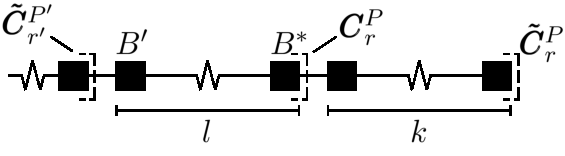
\includegraphics[width=0.5\columnwidth,keepaspectratio]{figures/longest-chain-proof.pdf}
    \caption{Longest chain recency proof. Block $B'$ is illustrated in the
             earliest possible position.
    }
   \label{fig:longest-chain-recency-proof}
  \end{figure}

  On the other hand, by Inequality~\ref{eq:bitcoin-r-bound}, $r - (r' + 2) \geq w - 1 \geq s$ and
  we can apply Chain Growth between rounds $r' + 2$ and $r$
  with parameters $s, \tau$ to obtain
  $|\TChain[][P][r]| - |\HChain[][P][r' + 2]| \geq \tau(r - (r' + 2)) \geq \tau (w - 1) \geq  k + \ell$,
  which is a contradiction because of Inequality~(\ref{eq:bitcoin-contradiction}).
  \Qed
\end{proof}

Ouroboros is already a Temporal Blockchain protocol with consistent recorded rounds.
The Bitcoin Backbone protocol can be augmented in a
straightforward manner to include recorded rounds, as done in the real Bitcoin deployment~\cite{mastering-bitcoin}.
The augmentation is illustrated in Figure~\ref{fig.temporal-backbone}.
The construction retains Common Prefix, Chain Quality and Chain Growth.
Furthermore, it has consistent recorded rounds.

\begin{figure}
  \begin{mdframed}
    The Temporal Bitcoin protocol is the Bitcoin protocol with
    the following additions:

    \begin{enumerate}
      \item Blocks include a round number. Genesis has recorded round $0$.
      \item Honest parties mine blocks with the current round.
      \item The recorded rounds of a valid chain are strictly increasing and not in the future.
    \end{enumerate}
  \end{mdframed}
  \caption{Temporal Bitcoin construction.}
  \label{fig.temporal-backbone}
\end{figure}

\begin{corollary}[Bitcoin and Ouroboros Timeliness]
  A typical execution of Temporal Bitcoin or Ouroboros is timely with parameter
  $v = \max(s, \frac{k + \ell}{\tau}) + 1$.
\end{corollary}
\begin{proof}
  Safety follows from Chain safety, which follows from Common Prefix~\cite[Theorem 15]{backbone}~\cite[Theorem 4.31]{ouroboros}.
  From Chain Quality($\mu,\ell$)~\cite[Theorem 16]{backbone}~\cite[Lemma 4.19]{ouroboros},
  Chain Growth($\tau, s$)~\cite[Theorem 12]{backbone}~\cite[Lemma 4.22]{ouroboros}, and Theorem~\ref{lem.longest-chain-recency},
  the execution is recent($\max(s, \frac{k + \ell}{\tau}) + 1$).
  From recorded round consistency and Theorem~\ref{thm.recency-to-freshness}, it is
  fresh($\max(s, \frac{k + \ell}{\tau}) + 1$).
  From this, safety, recorded round consistency and Theorem~\ref{thm:freshness-to-timeliness},
  timeliness($\max(s, \frac{k + \ell}{\tau}) + 1$) follows.
  \Qed
\end{proof}